\subsection{UC3 - Scelta delle Labels}
\label{uc3}

    \begin{figure}[htbp]
        \centering
        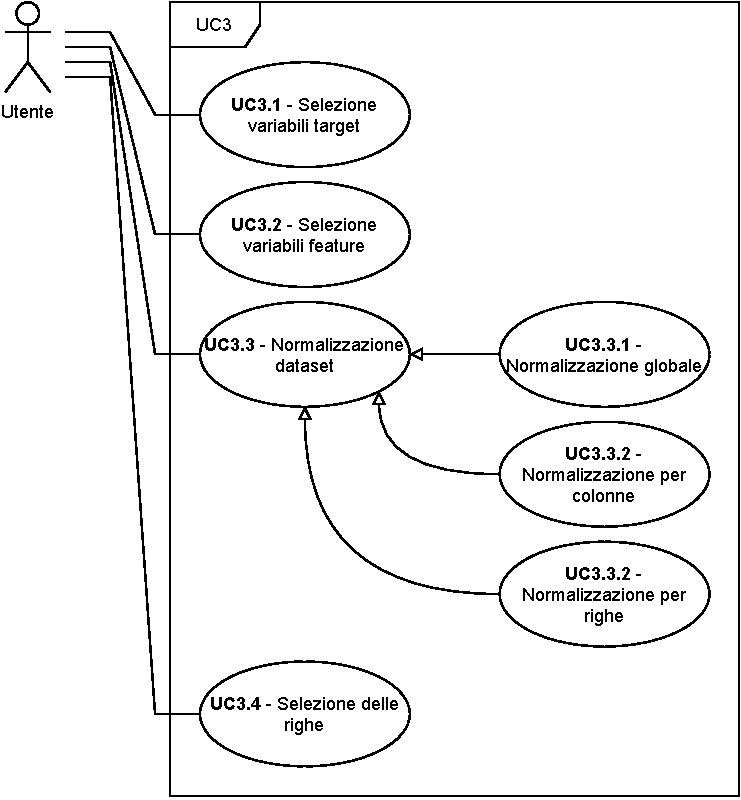
\includegraphics[width=0.5\textwidth]{source/sections/casi-uso/diagrams/uc3.pdf}
        \caption{UC3 - Scelta delle Labels}
        \label{fig:uc3}
    \end{figure}


    \begin{itemize}
    \item \textbf{Attore}: Utente
    \item \textbf{Descrizione}: Tra le dimensioni (colonne della matrice) del dataset caricato possono essere presenti delle labels, l'applicazione offre un meccanismo tramite cui l'utente può selezionare queste tipo di features e separarle dalle features numeriche che invece compongono le coordinate del dato $n$-dimensionale.
    \item \textbf{Precondizione}:
    \begin{itemize}
        \item Eseguito l'upload del dataset come matrice $N\times M$ (\hyperref[uc2]{UC2}).
        \item Selezionata una tra le visualizzazioni Scatter Plot Matrix (\hyperref[uc2.1]{UC2.1}), Force Field (\hyperref[uc2.4]{UC2.4}) Linear Projection (\hyperref[uc2.5]{UC2.5})
    \end{itemize}
    \item \textbf{Postcondizione}: Le features selezionate verranno considerate dal sistema come labels.
    \item \textbf{Scenario Principale}: 
    \begin{enumerate}
        \item L'utente visualizza le features del dataset.
        \item Seleziona le features del dato che ritiene essere delle labels.
    \end{enumerate}  
    \end{itemize}
    
    \subsubsection{UC3.1 - Assegnazione delle classi di visualizzazione alle Labels}
    \label{uc3.1}
    \begin{itemize}
    \item \textbf{Attore}: Utente
    \item \textbf{Descrizione}: L'utente decide di assegnare dei diversi modi per distinguere un punto nel grafico, assegnando una classe di visualizzazione (colore, forma, size) ad ogni label, in questo modo risulta più semplice per l'analista vedere dei pattern nella visualizzazione del grafico.
    \item \textbf{Precondizione}:
    \begin{itemize}
        \item Eseguito l'upload del dataset come matrice $N\times M$ (\hyperref[uc2]{UC2}).
        \item Selezionato una tra le visualizzazioni Scatter Plot Matrix (\hyperref[uc2.1]{UC2.1}), Force Field (\hyperref[uc2.4]{UC2.4}) Linear Projection (\hyperref[uc2.5]{UC2.5}).
        \item Nel dataset, almeno una feature è stata selezionata come label.
    \end{itemize}
    \item \textbf{Postcondizione}: Al variare del valore della etichetta $X$, i punti visualizzati assumono un diverso attributo della classe assegnata a quest'ultima.
    \item \textbf{Scenario Principale}: 
    \begin{enumerate}
        \item L'utente visualizza tutte le labels selezionate.
        \item L'utente associa ad ogni label una classe di visualizzazione.
    \end{enumerate}  
    \end{itemize}